% Chapter 6

\chapter{Conclusions} % Main chapter title

\begin{figure}[hbtp]

\centering
    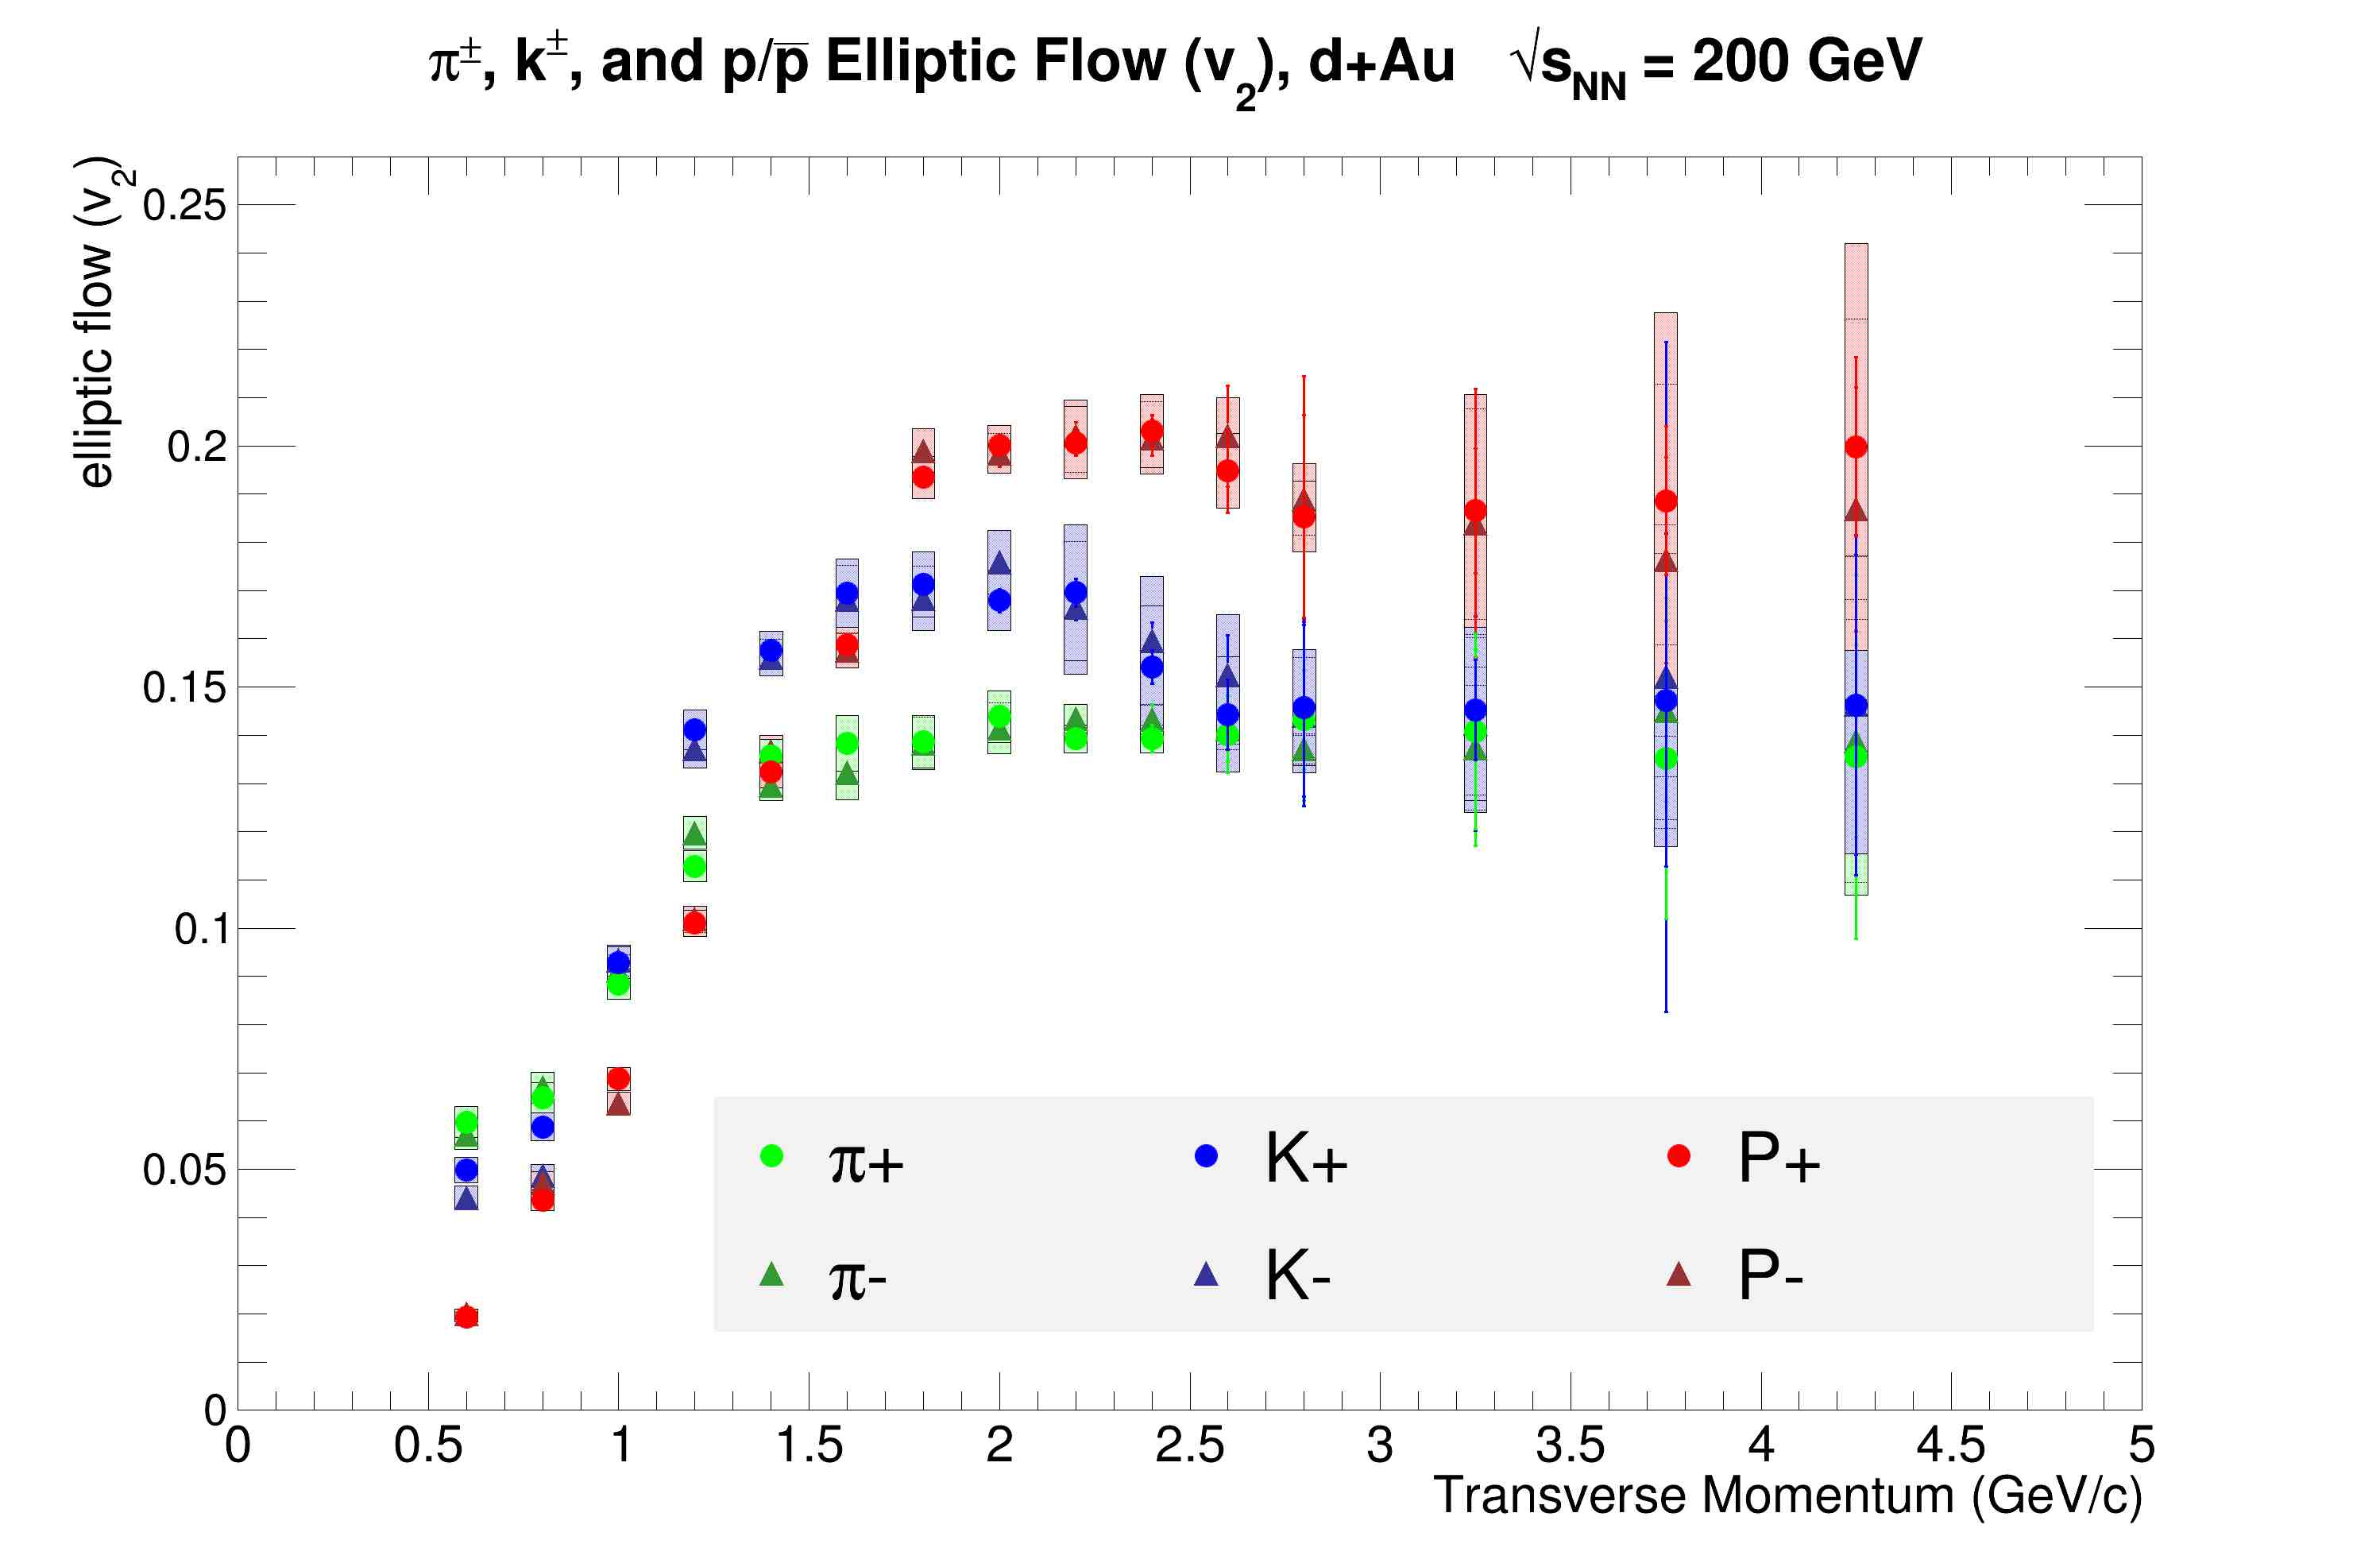
\includegraphics[width=0.7\textwidth]{results/v2all.jpg}
    \rule{35em}{0.5pt}
    \caption[Elliptic Flow vs Transverse Momentum, 200 GeV d+Au]{Elliptic Flow vs Transverse Momentum, 200 GeV d+Au}
    \label{fig:v2main}
\end{figure}

Measurements of the second Fourier coefficient corresponding to an elliptically shaped azimuthal anisotropy of pions, kaons, and (anti)protons produced in 200 GeV deuteron-gold collisions are presented in figure \ref{fig:v2main}. This measurement is a sign that collective behavior happens in systems previously thought of as ``cold'' and is an indication that a QGP could be formed in the simpler system of d+Au. This flow increases steadily for all hadrons up to $p_T \sim 1.5 $ GeV/c where the mesons (pions and kaons) seem to reach a saturation and flatten out. The kaons exhibit a flow signal stronger than the pions in this range but eventually decreasing to the same nominal value as the pions. The (anti)protons continue to flow increasingly up to $p_T \sim 2$ GeV/c. 

\section{Discussion}

\subsection{Hadronization}
\begin{figure}[hbtp]
\centering    
    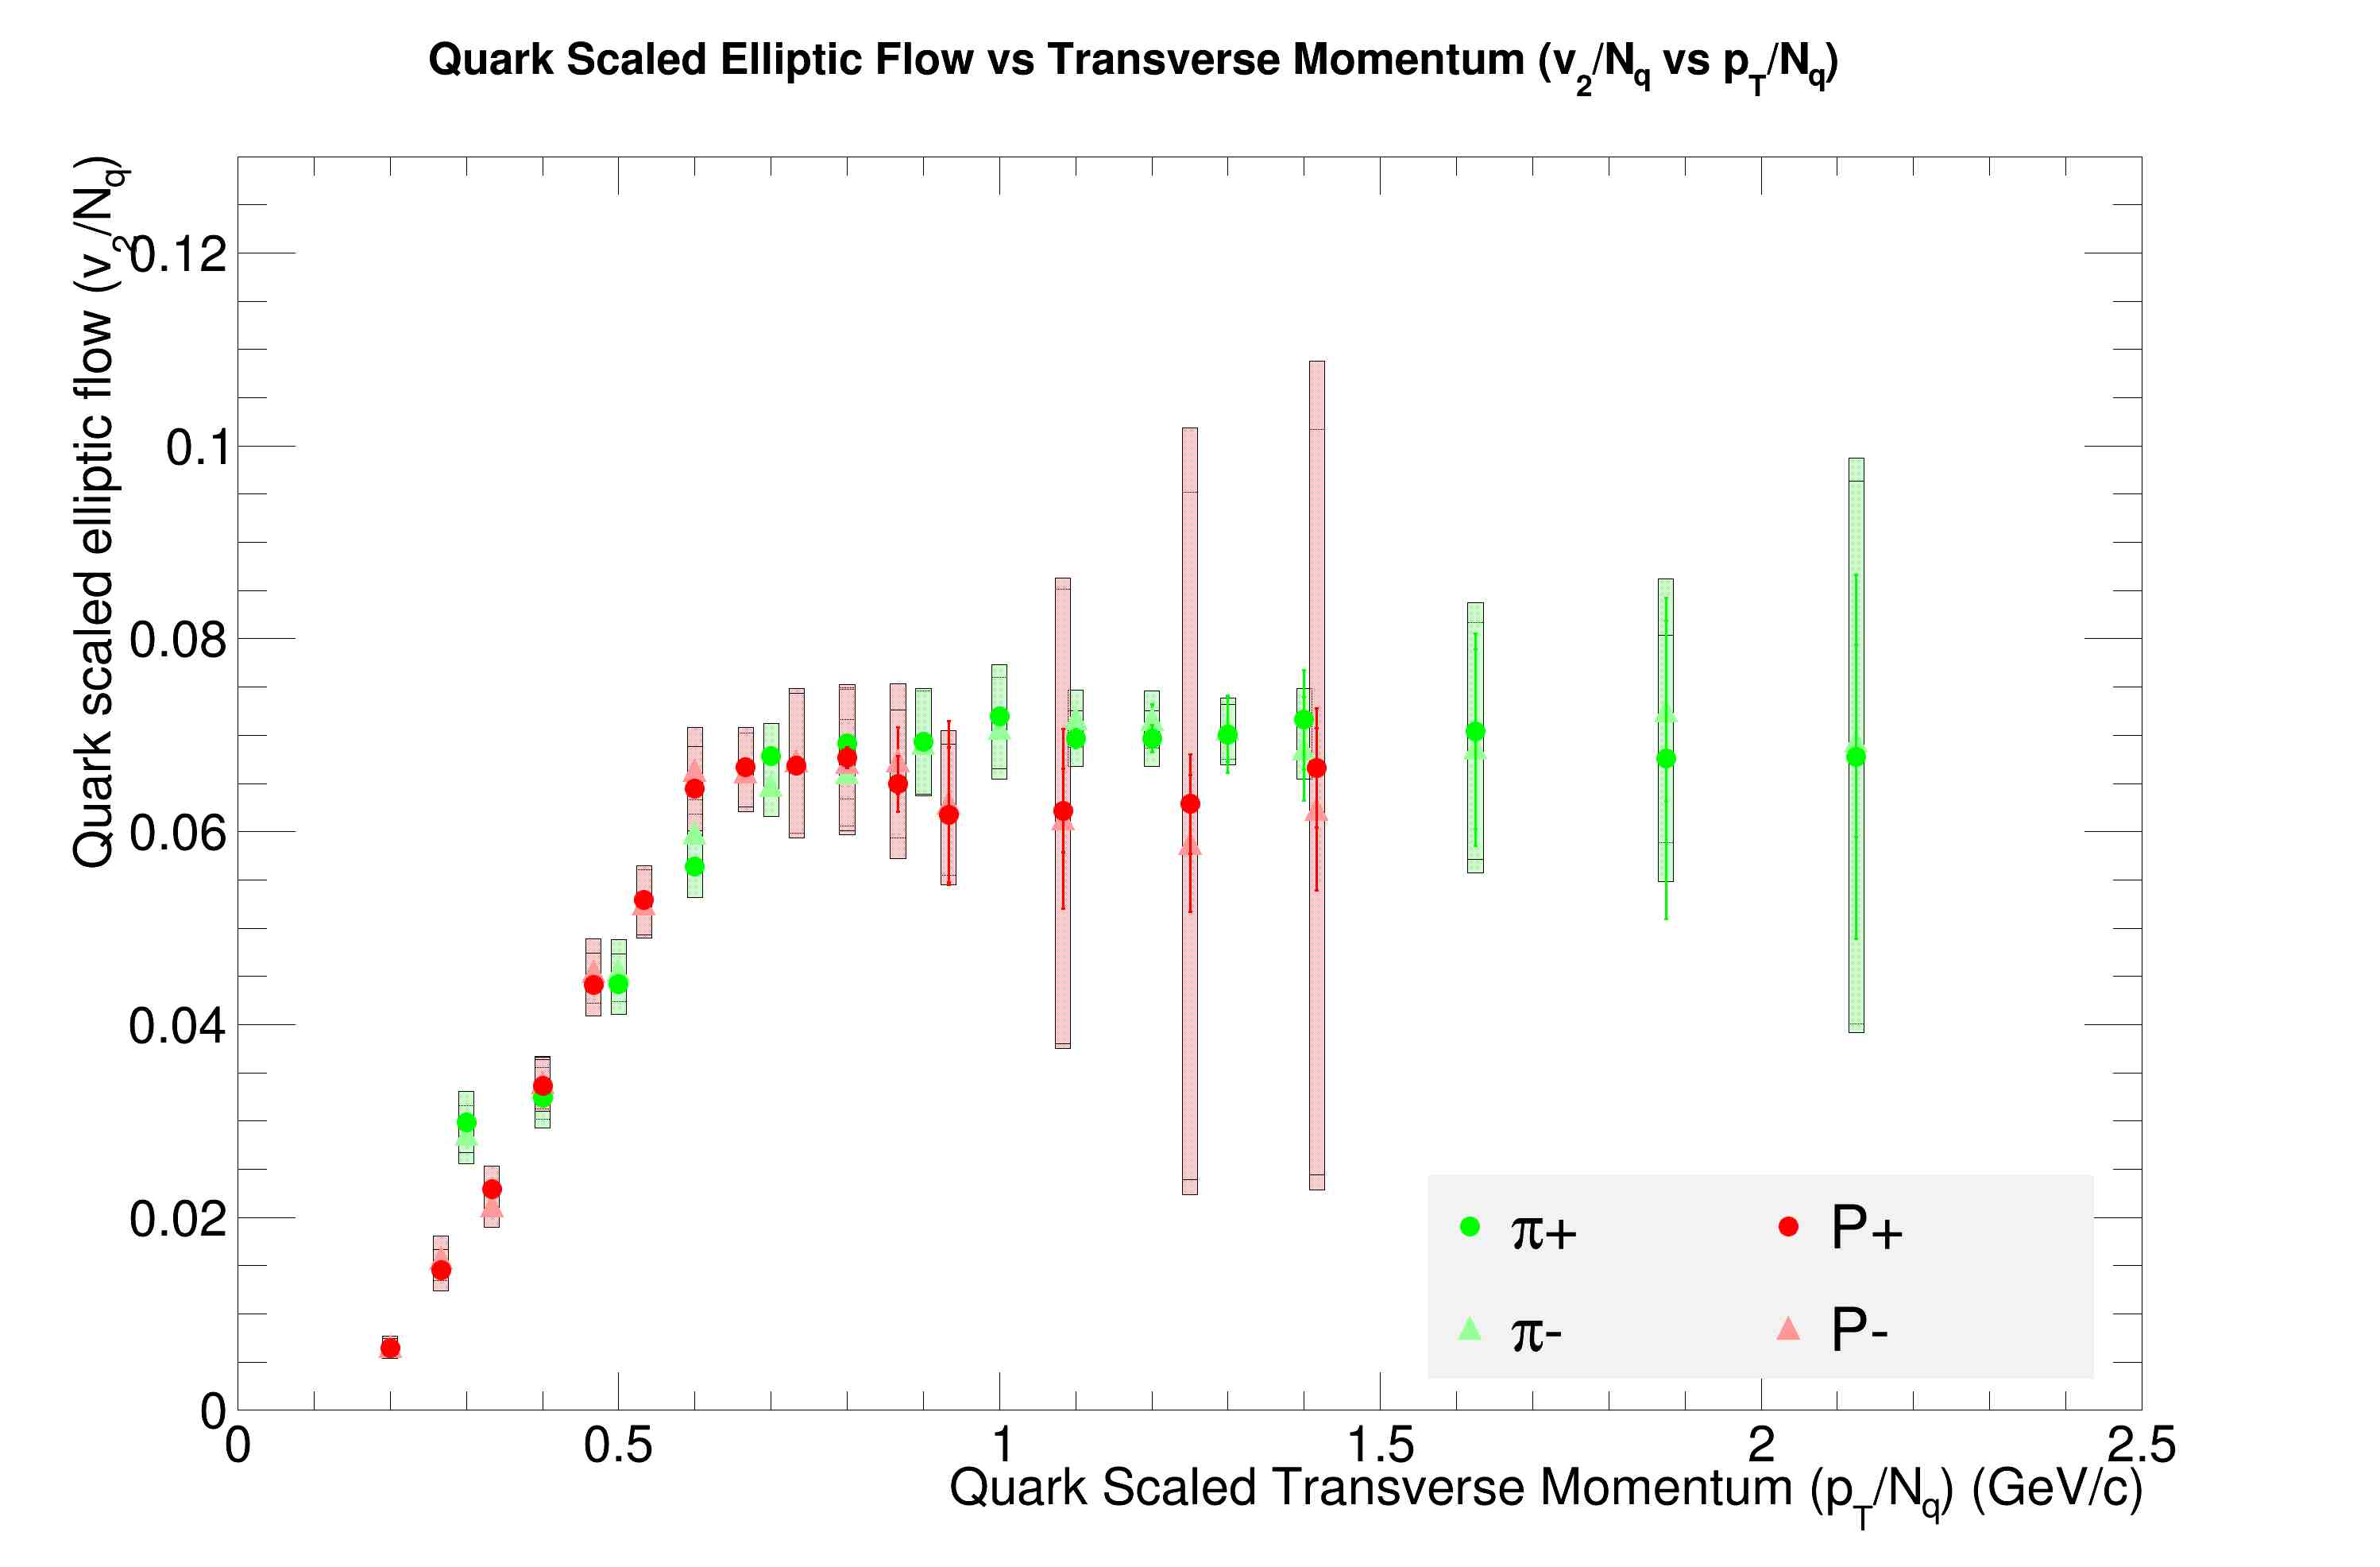
\includegraphics[width=0.7\textwidth]{results/v2NqvspT.jpg}
    \rule{35em}{0.5pt}
    \caption[Quark Scaled Elliptic Flow ($\pi^{\pm}$ and $p/\bar{p}$) vs Transverse Momentum, 200 GeV d+Au]{Quark Scaled Elliptic Flow ($\pi^{\pm}$ and $p/\bar{p}$) vs Transverse Momentum, 200 GeV d+Au}
    \label{fig:qscaledv2}
\end{figure}

This (anti)proton flow enhancement in the mid-$p_T$ range is similar to the baryon enhancement seen in previous experiments. Assuming quark deconfinement is achieved (which collective flow is a strong indicator of), this enhancement must happen in the freeze out stage. The leading model describing this phenomenon, recombination/fragmentation, can be seen by scaling the flow coefficient and momentum by the number of quarks that comprise the measured particle\footnote{2 quarks for pions/kaons, 3 quarks for protons}. Doing so shows that this particle momentum discrepancy may come from the sum of momenta of the constituent quarks. That is to say, the reason why protons appear to have stronger flow is simply because they contain more quarks. For example, if we were to take three quarks that have the same momentum, they would combine to produce a particle with higher momentum than if only two of those quarks had combined. This quark scaled flow is shown in figure \ref{fig:qscaledv2} for pions and protons and shows that both particle signals increase and reach saturation in the same range. This is a strong indication of recombination as the mechanism for thermal freeze-out and is a result that agrees with similar quark scaled results in $^3$He+Au\citep{huangQM2015}, Au+Au\citep{Adler:2003kt}, Cu+Cu\citep{PhysRevC.92.034913}, Pb+Pb\citep{Noferini:2012ps} systems both at RHIC and abroad.

\subsection{Comparison to Flow Models}
\begin{figure}[hbtp]
\centering    
    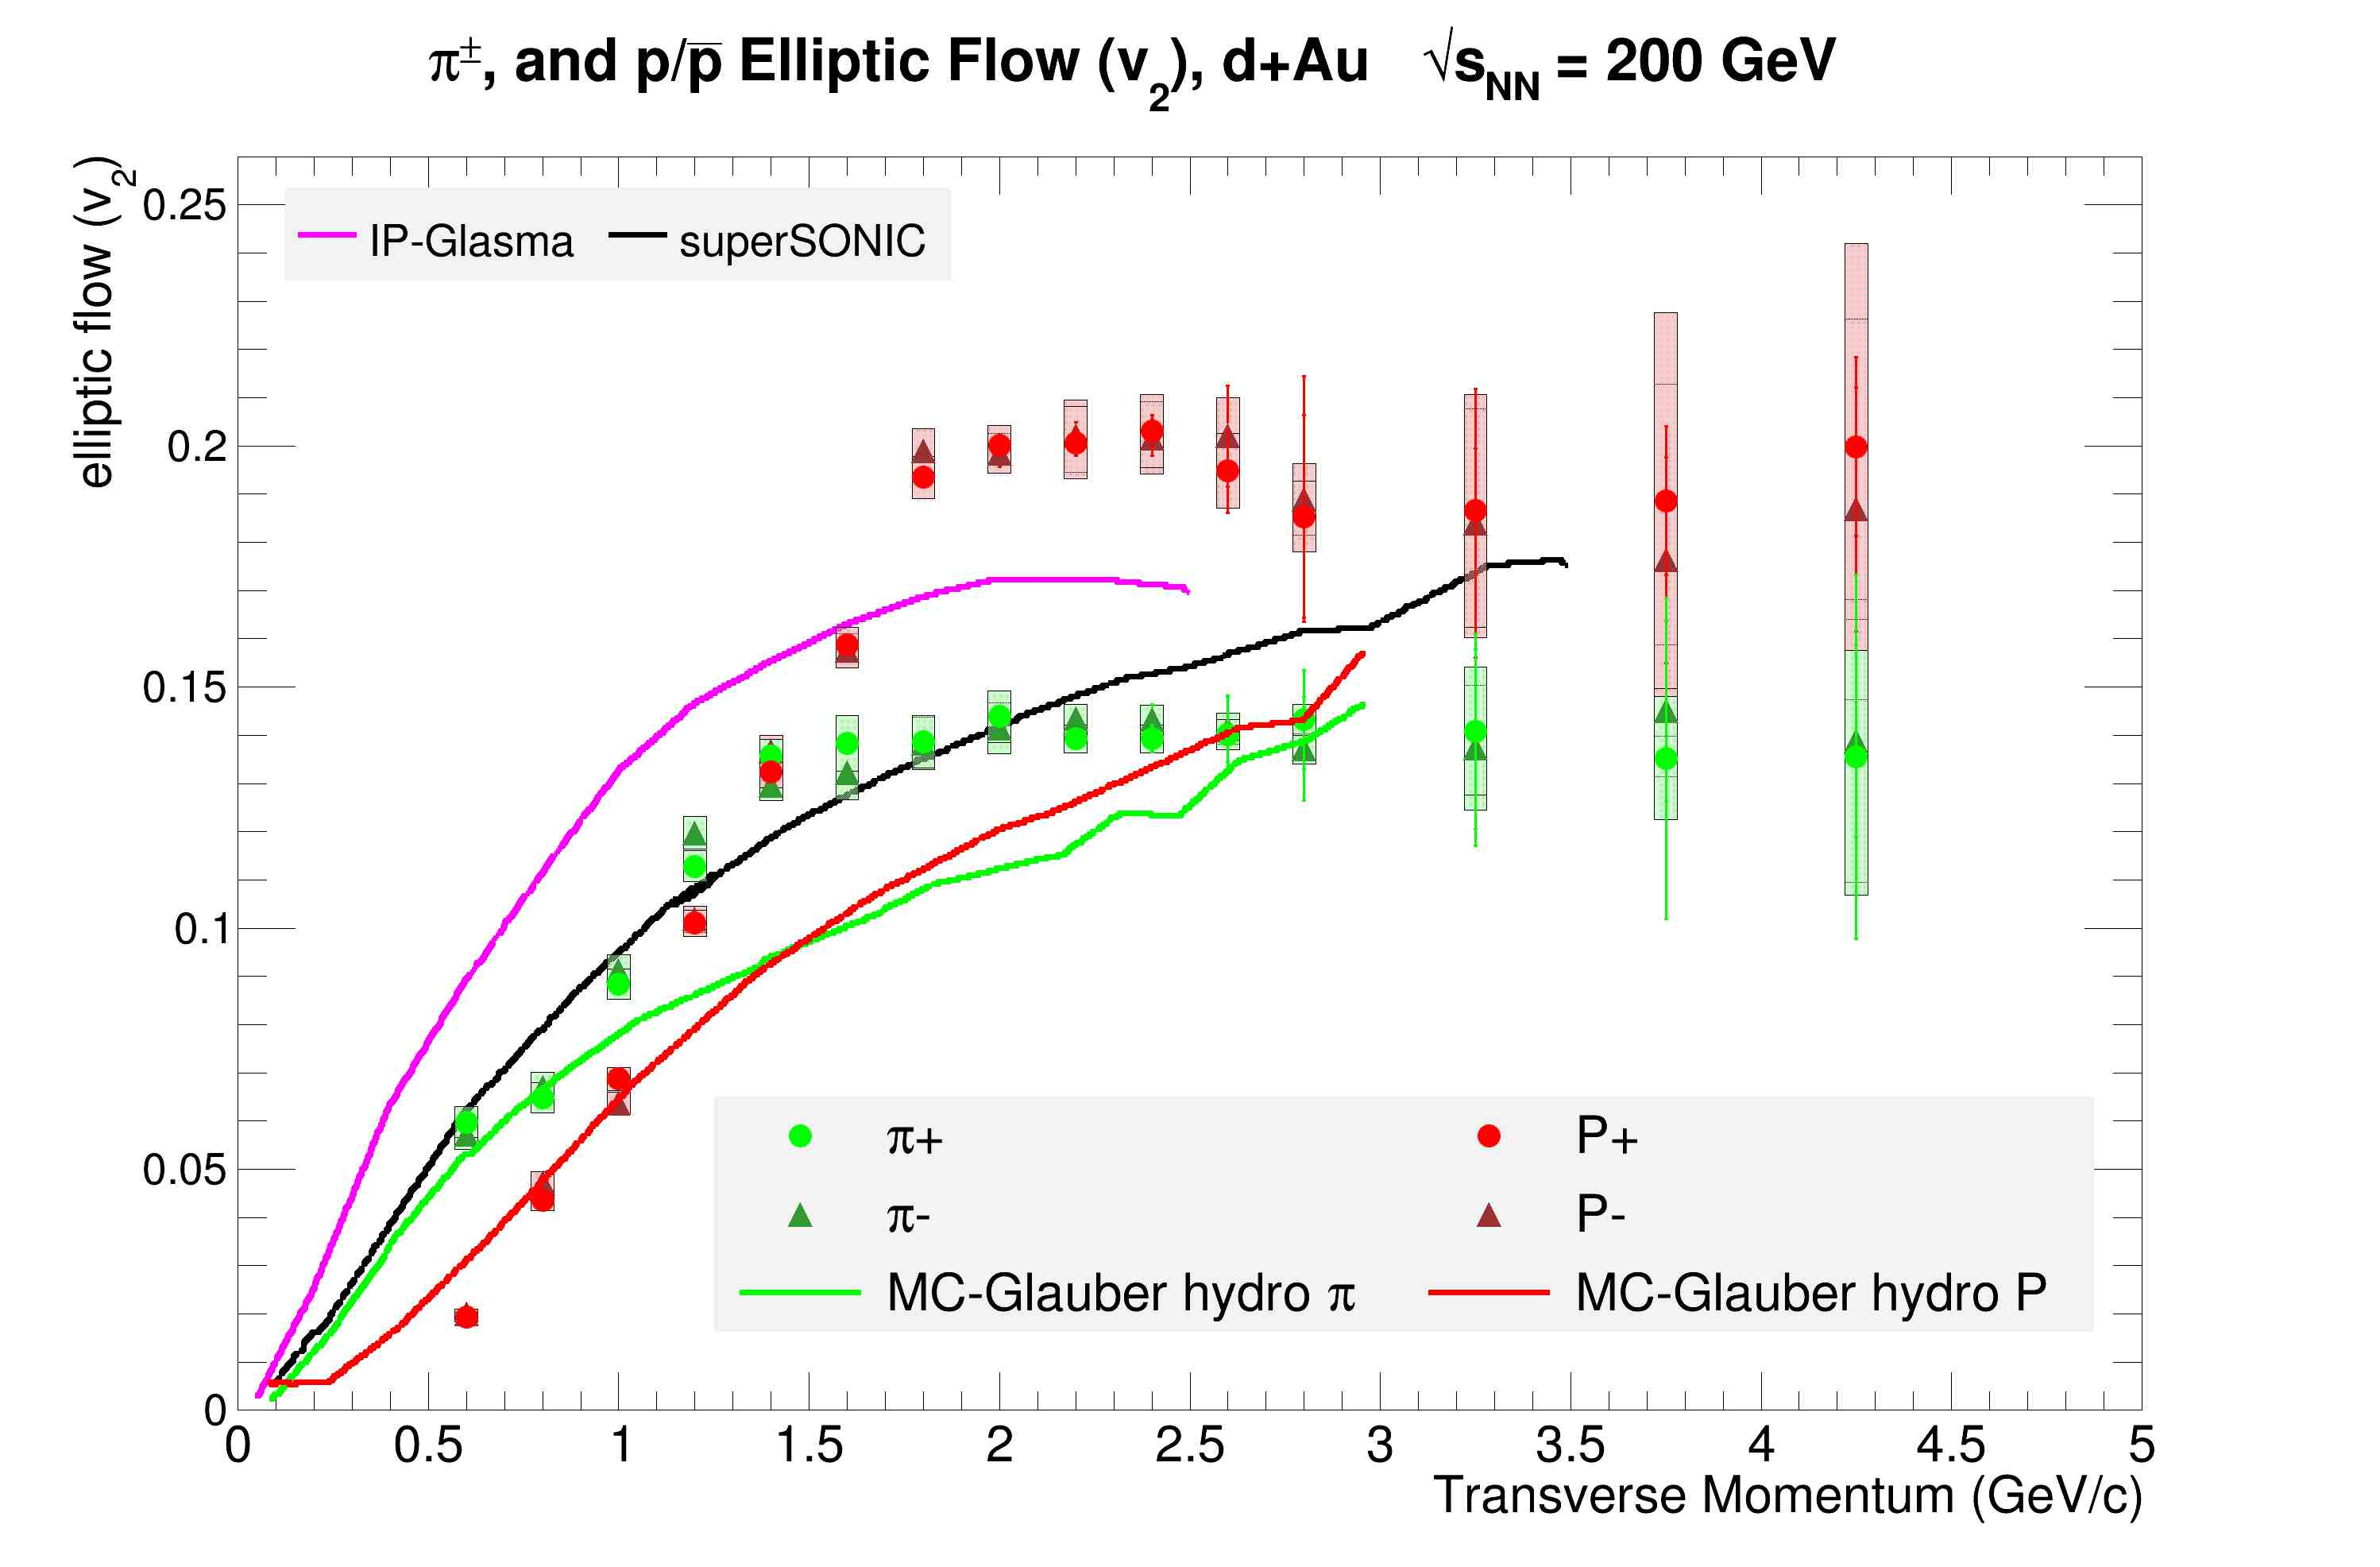
\includegraphics[width=0.7\textwidth]{results/v2allpipmodels.jpg}
    \rule{35em}{0.5pt}
    \caption[$\pi^{\pm}$ and $p/\bar{p}$ Elliptic Flow compared to hydrodynamic models.]{$\pi^{\pm}$ and $p/\bar{p}$ Elliptic Flow compared to hydrodynamic models: MC-Glauber\citep{Nagle:2013lja}, IP-Glasma\citep{Schenke:2014gaa}, and superSONIC\citep{Romatschke2015}}.
    \label{fig:hydrov2}
\end{figure}

Prior to hadronization, the equilibrated state of deconfined quarks has been described well with viscous hydrodynamic models. The way these models differ is in their assumption of the initial conditions (Glauber versus CGC) and duration of equilibration time. A comparison of this measurement with these hydrodynamic models is shown in figure \ref{fig:hydrov2}. Models using Monte Carlo simulations of identified particle flow that utilize Glauber initial conditions (MC-Glauber) describe the data well for low $p_T$ but diverge above $p_T \sim 1$ GeV/c, also seen in d+Au in a previous PHENIX analysis\citep{Adare:2014keg}\footnote{though diverging at slightly higher transverse momentum, $p_T < 1.5 $GeV/c}. A continuation of MC-Glauber including a longer equilibration time (longer period of \textit{pre-flow} before a thermalized QGP flow) and the effect of post freeze-out hadron interaction\footnote{referred to in literature as \textit{Hadronic Cascade Afterburner}} called \textit{superSONIC}\citep{Romatschke2015}\footnote{an extension of an earlier SONIC model with a longer pre-flow time. SONIC stands for \textit{Super hybrid mOdel simulatioN for relativistic heavy-Ion Collisions}\citep{Romatschke2015}} matches data up to higher $p_T$ but does not match the flow signal's saturation that begins just below $p_T \sim 2$ GeV/c, an effect also seen in the aformentioned PHENIX d+Au analysis. A model using impact parameter independent CGC/Glasma (IP-Glasma)\citep{Schenke:2014gaa} as an initial condition overestimates the flow strength but does appear to model the asymptotic flow behavior at mid-high $p_T$, albeit overestimating the the value of that maximum flow value slightly. To minimize the effect of baryon enhancement in mid $p_T$, the elliptic flow of all hadrons is approximated by summing the yields of all identified tracks and performing a flow analysis. This is shown compared to both IP-Glasma and superSONIC models in figure \ref{fig:allhadronhydro}
\begin{figure}[hbtp]
\centering    
    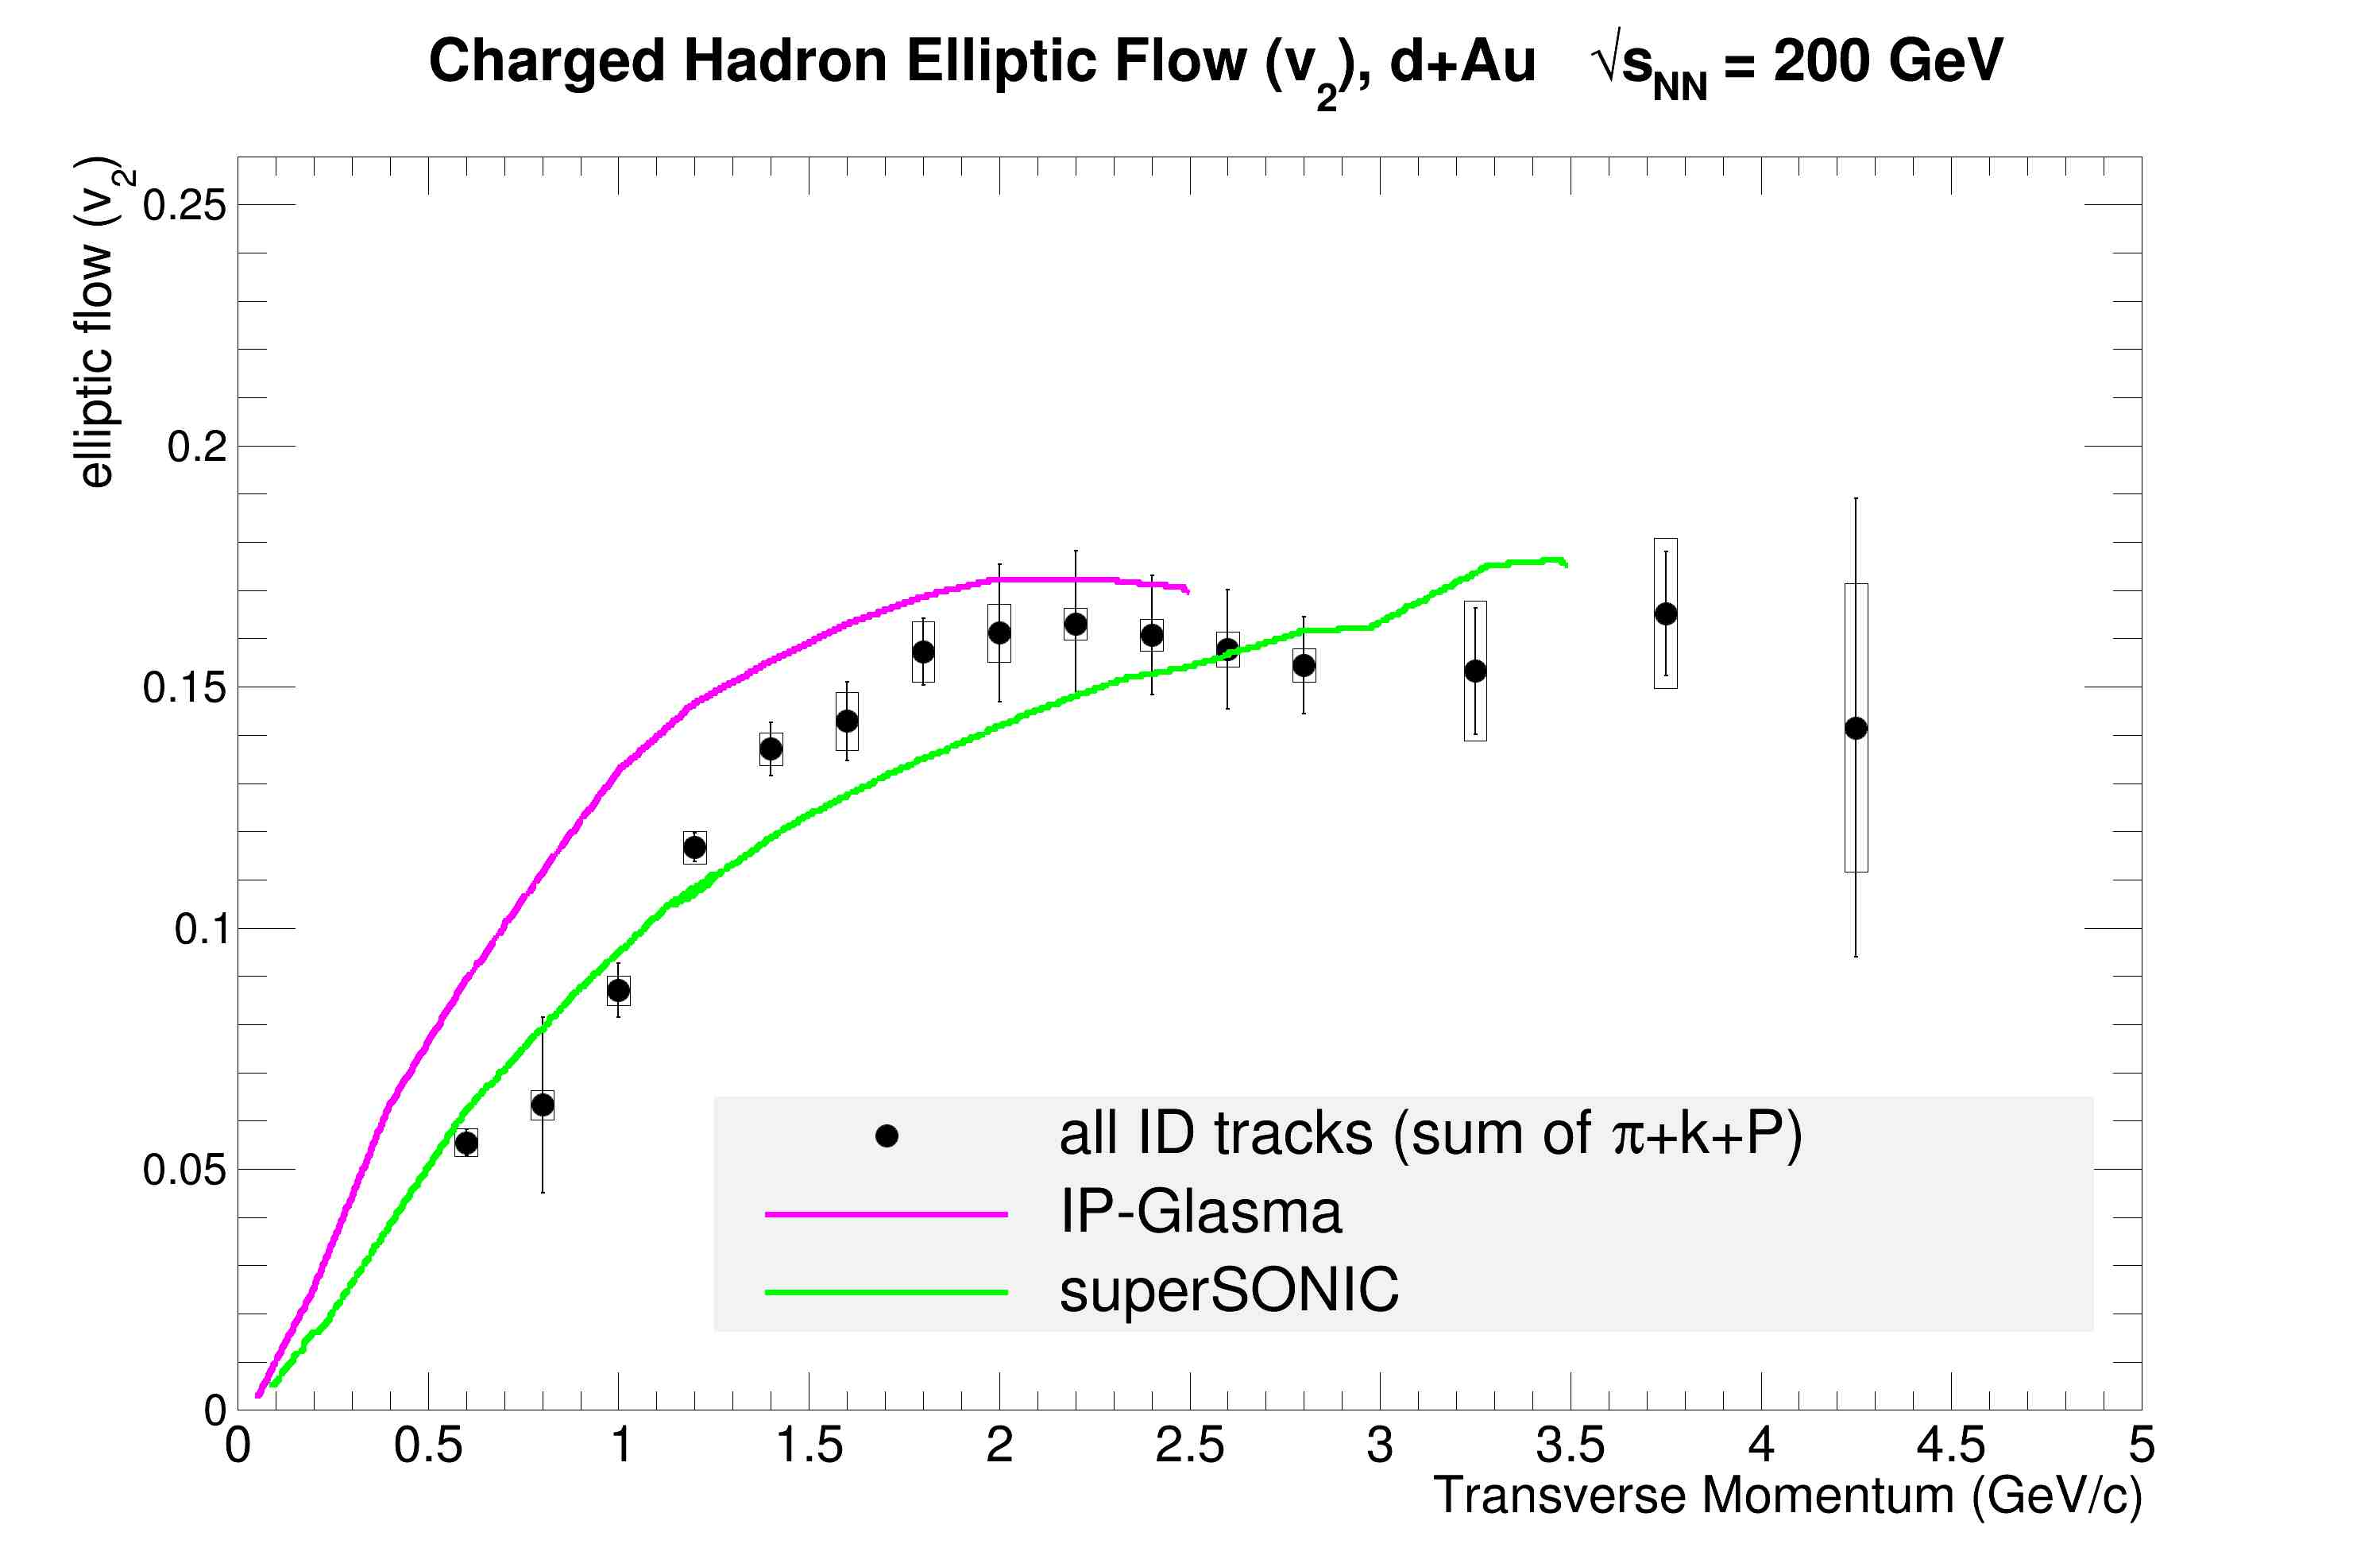
\includegraphics[width=0.7\textwidth]{results/v2hydro.jpg}
    \rule{35em}{0.5pt}
    \caption[Elliptic flow of all charged hadrons compared to hydrodynamic models.]{Elliptic flow of all charged hadrons measured by summing the yields of all identified tracks. Data is compared to IP-Glasma and superSONIC models.}.
    \label{fig:fig:allhadronhydro}
\end{figure}

\subsection{Strangeness and Initial Conditions}





\pagebreak
\pagebreak


